
%
\documentclass[runningheads]{llncs}
\usepackage{graphicx}
\usepackage{amsmath,amsfonts,amssymb}
\usepackage{array,booktabs}
\usepackage{parskip}
\usepackage{mathtools}
\usepackage{subfig}
%
\begin{document}
% title
\title{Nonlinear and Chaotic Pendulum Simulations Using Lagrangian Mechanics}
%\thanks{Supported by Mult x.} % if we want to thank someone/org.
%
% authors
\author{Timothy Holmes}
%
\authorrunning{Timothy Holmes}
% First names are abbreviated in the running head.
%
\institute{{DePaul University Department of Physics}}
%
\maketitle              % typeset the header of the contribution
%
Many classical systems can be solved using Newtonian mechanics. However, when solving for more complex systems Newtonian mechanics are not necessarily ideal and becomes difficult to solve the problem. Lagrangian mechanics through the use of generalized coordinates and conservation laws will reduce the system into differential equations for the classical system. These differential equations are physically know as the equations of motion for the system. The equations of motion describe the behavior of the physical system over time. Once the equations of motion are found using the Euler-Lagrange equation, the motion of the system can be better understood. Without computational power the in-site on the motion of the is limited. Modeling a differential equation can give better in-site on how the system actually works, allows for quick variation of parameters, different initial conditions, and so forth. Solving a complicated system just like the double pendulum would become very hard to understand and becomes easier when solving for it numerically. The Lagrangian of the double pendulum is given by

\begin{multline}
    L = \frac{1}{2}(m_{1} + m_{2}) \ell_{1}^{2}\dot{\theta_{1}}^{2} + \frac{1}{2}m_{2}\ell_{2}^{2}\dot{\theta_{2}}^{2} + m_{2}\ell_{1}\ell_{2}  \dot{\theta_{1}}\dot{\theta_{2}}cos(\theta_{1} - \theta_{2})\\ + (m_1 + m_2)g\ell_{1}cos(\theta_{1}) + m_{2}g\ell_{2}cos(\theta_{2}).
\end{multline}

Since there are two different $\theta$ term, there are two different equations of motion. The equations of motion for this Lagrangian are much longer than the Lagrangian itself. It becomes apparent for a complex system like this that computationally solving it make understanding the problem much more straightforward.  

\begin{figure}[h!]
    \centering
    \subfloat[Pendulum mass path]{{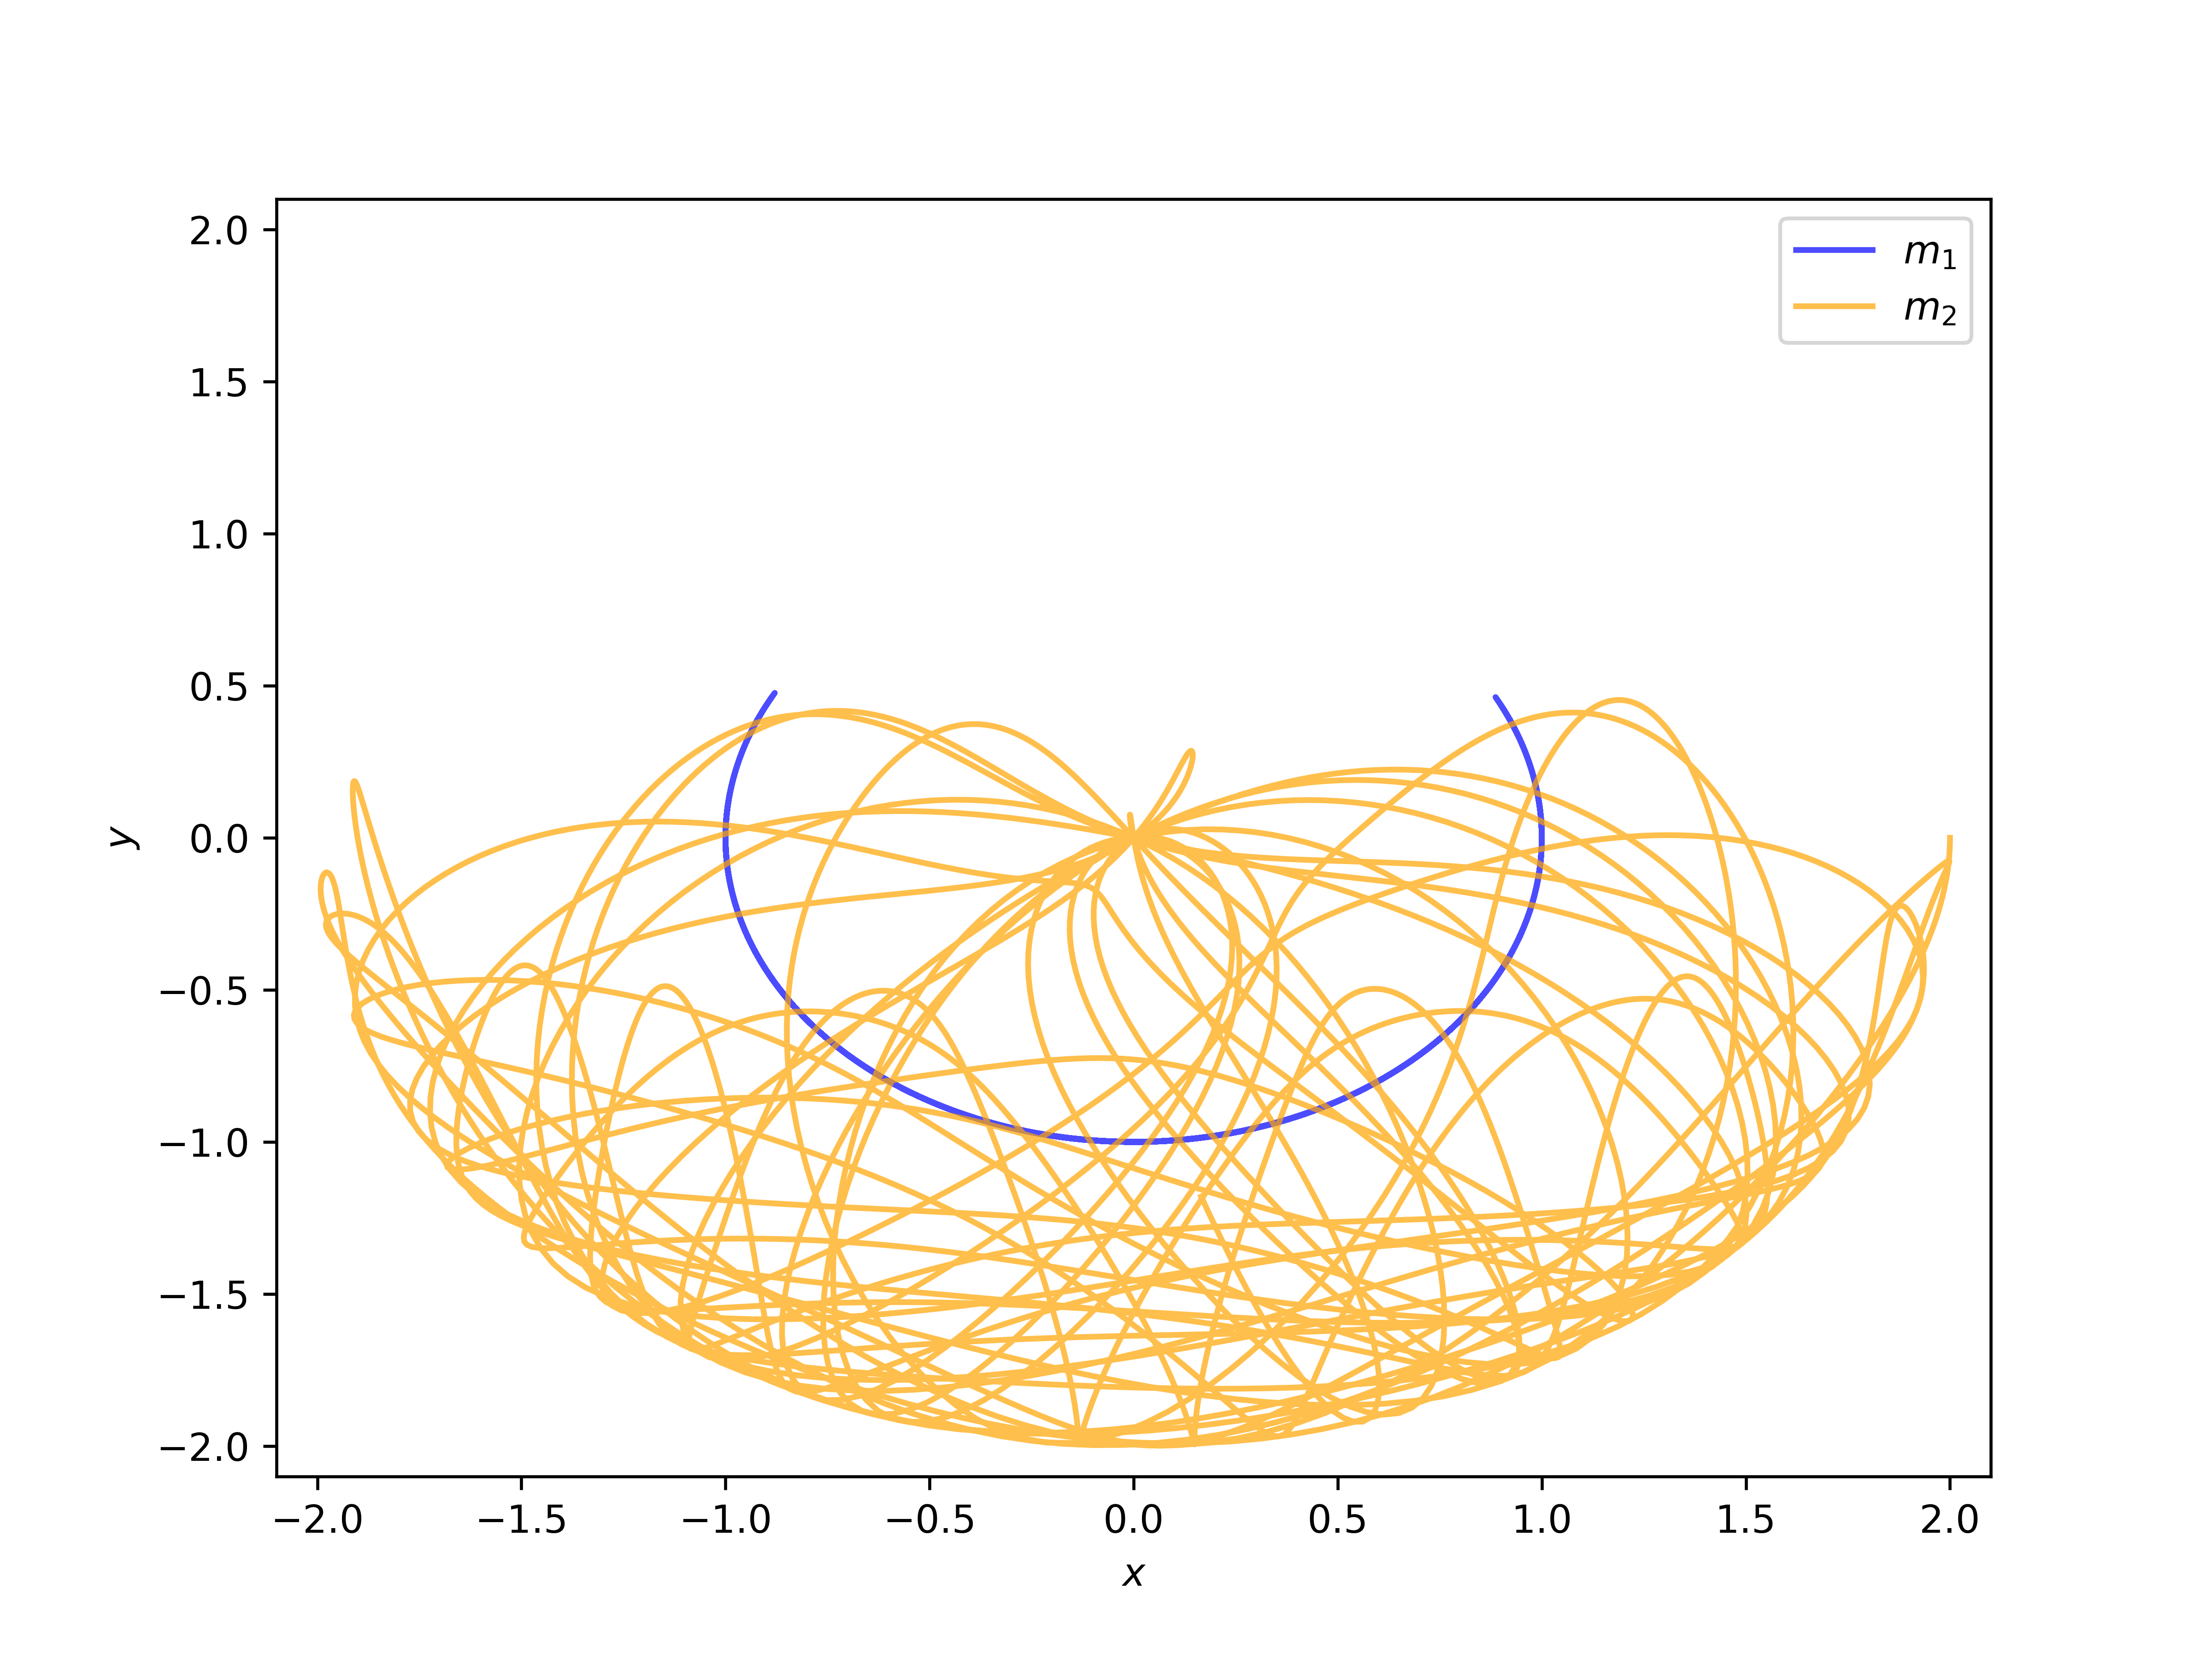
\includegraphics[width=4cm]{img/double_pendulum_path_pi2.png} }}%
    \qquad
    \subfloat[Double pendulum $\theta_{1}$ and $\theta_{2}$ over time]{{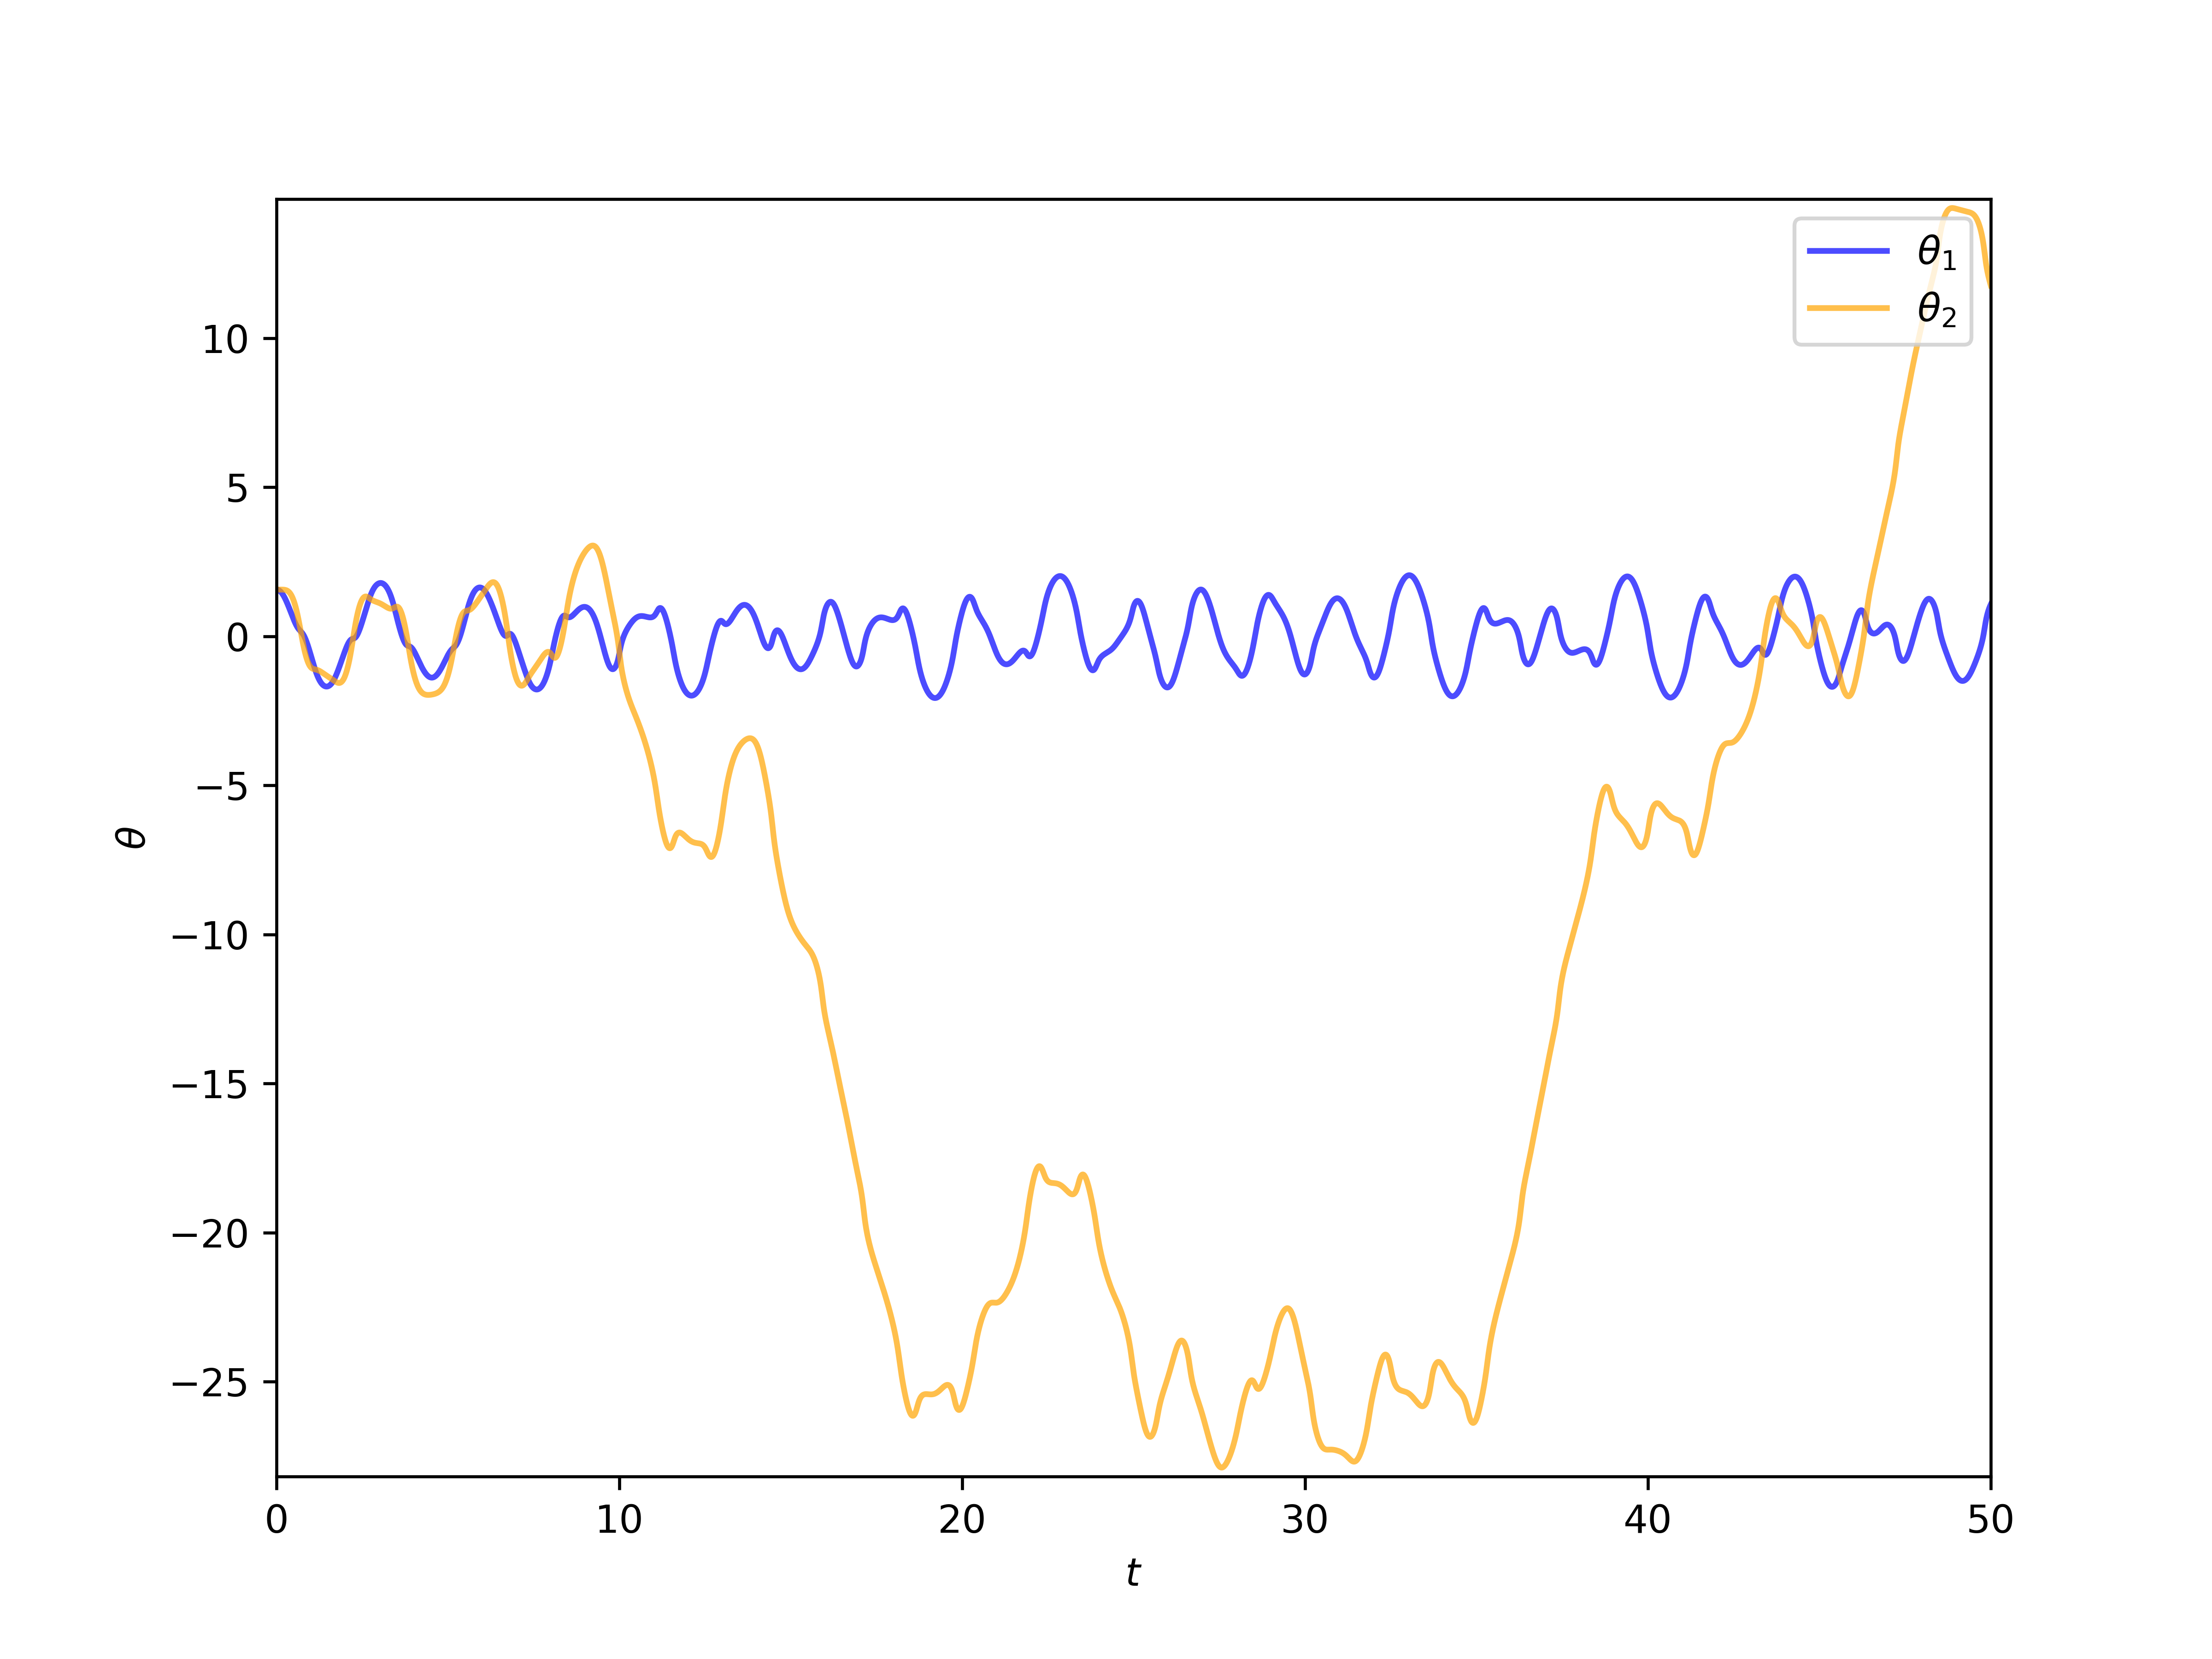
\includegraphics[width=4cm]{img/double_pendulum_angle_pi2.png} }}%
    \caption{The double pendulum model with large initial angles}%
    \label{fig:example}%
\end{figure}

Figure 1 is an example of some of the information you can find by numerically solving the differential equation. This output from the model makes it simple to see how chaotic the motion of a double pendulum can be. On the other hand modeling a simple pendulum will show how predictable the equation of motion is. \\

The method of solving these with a computer is the same as solving by hand. First find the kinetic energy and potential energy of the system. Find the coordinate transformations. Set up the Lagrangian and use the Euler-Lagrange equation to find the equation of motion. Use a numerical method to solve the differential equation and animate.

\end{document}